\section{Evaluation of the ABSNF}
\subsection{Problem Specification}

ABS-Normal Form:
\begin{flalign*}
\begin{pmatrix}
\Delta z \\
\Delta y
\end{pmatrix}
= 
\begin{pmatrix}
a \\
b
\end{pmatrix}
+
\begin{pmatrix}
Z & L \\
J & Y 
\end{pmatrix}
\circ
\begin{pmatrix}
\Delta x \\
|\Delta z |
\end{pmatrix}
\end{flalign*}
Given is a PL function in abs-nf. The evaluation of this function means calculating the vectors $\Delta y$ and $\Delta z$:
\begin{flalign}
\Delta y &= b + (J \times \Delta x) + (Y \times |\Delta z|) \label{eval_1}\\
\Delta z &= a + (Z \times \Delta x) + (L \times |\Delta z|) \label{eval_2}
\end{flalign}
where the following structures are given:
\begin{flalign*}
a,b,Z,L,J,Y,m,n,s, \Delta x
\end{flalign*}
In (\ref{eval_2}) $\Delta z$ depends on the element-wise absolute function of its own and therefore it cannot be calculated with a simple matrix vector dot product. Since the matrix $L$ is lower triangular, the vector $\Delta z$ can be iteratively calculated, by taking the row-wise dot product of $L$ and $|\Delta z|$. \\

\begin{flalign*}
k = a + Z \times \Delta x
\end{flalign*}

\begin{flalign*}
\highlightblue{\Delta  z_1}  &= \underbrace{L_1 \times |\Delta z|}_{=0} + k_1 = k_1 \\
\highlightyellow{\Delta z_2} &= L_2 \times |\Delta z| + k_2 \\
	&= L_{2,1} \times \highlightblue{|\Delta z_1 |} + k_2 \\
\highlightgreen{\Delta z_3} &= L_3 \times |\Delta z| + k_3 \\
	&= L_{3,1} \times \highlightblue{|\Delta z_1 |} + L_{3,2} \times \highlightyellow{|\Delta z_2|} + k_3 \\
\highlightred{\Delta z_4} &= L_{4} \times |\Delta z| + k_4 \\
	&= L_{4,1} \times \highlightblue{|\Delta z_1|} + 
	L_{4,2} \times \highlightyellow{|\Delta z_2|} +
	L_{4,3} \times \highlightgreen{|\Delta z_3|} + k_4 \\
	....
\end{flalign*}

\subsection{Implementation}
Our implementation is highly focused on speed and  demands the device to hold all the required data structures in global memory simultaneously. \\

Given this premise, the calculation of (\ref{eval_1}) and (\ref{eval_2}) is a series of dot products and therefore is highly parallelize-able. For this we relied mainly on CUBLAS routines. The implementation is available on [...] with several interfaces in [...]..

\begin{lstlisting}[language=cpp]
template <typename T>
void eval(T *a, T *b, 
T *Z, T *L, 
T *J, T *Y,
T *dx,
int m, int n, int s,
T *dz, T *dy,
T *abs_dz)
{
// dz = a
cudaMemcpy(dz, a, ., cudaMemcpyDeviceToDevice));
// dz = Z * dx + dx
cublasDgemv(.,Z, ., dx, . dz, .)
// dz[i] = L[i]_i * |dz|_i
for(int i=0; i<s; i++)
{
cublasDgemv( . ,&L[i * s], . ,abs_dz, . , &dz[i],.);
abs <<<1,1>>>(&dz[i], &abs_dz[i], 1);
}
// dy = b
cudaMemcpy(dy, b, ., cudaMemcpyDeviceToDevice);
// dy = dy + J*dx
cublasDgemv(.,J, ., dx, ., dy, .));
// dy = dy + Y * |dz|
cublasDgemv(., Y, ., abs_dz, ., dy, .));
}
\end{lstlisting}

\subsubsection{Performance Experiments}
For measuring performance and the subsequent analysis, we simplified the process by equalizing the dimensions of the data-structures:
\begin{flalign*}
	m = n = s
\end{flalign*}

\subsubsection{Single Execution}

In this experiment, we executed the serial python implementation as well as the parallel cuda implementation for different dimensions of $s$ and measured the total runtime of the program. The results can be seen in figure \ref{eval_single_repetition}. Since the results were not as expected in favor of the CUDA implementation, we also dismantled the runtime on the parallel devices and measured the "data-upload-time" and the "execution-time" separately. Those results can be found in figure \ref{eval_memory}. Here we can clearly see, that the transfer time, which is the time that it takes to upload the required datastaructures onto the device is extremely significant and takes a disproportional high share of the total time.

\begin{figure}[ht]
	\centering
	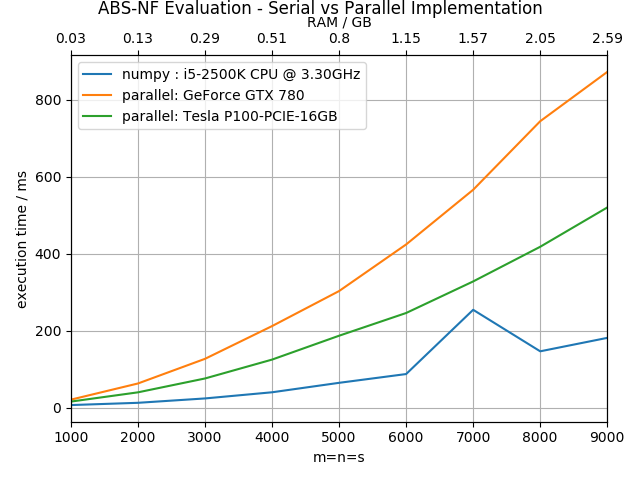
\includegraphics[width=0.6\textwidth]{img/eval_single_repetition.png}
	\caption{Single execution of the evaluation function on different devices.}
	\label{eval_single_repetition}
\end{figure}

\begin{figure}[ht]
	\centering
	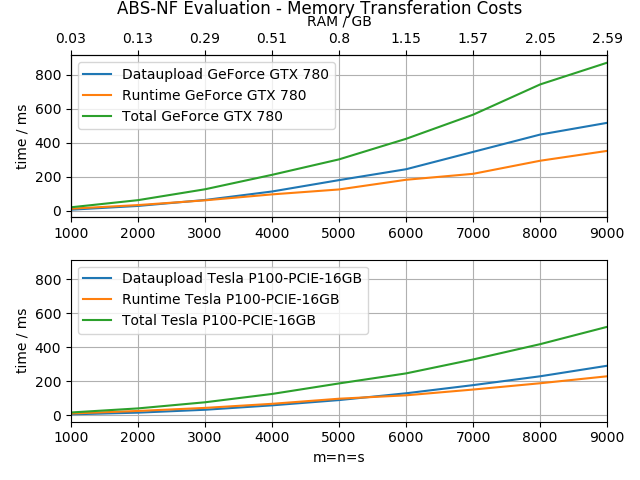
\includegraphics[width=0.6\textwidth]{img/eval_memory.png}
	\caption{Datatransfer and execution time of the parallel implementation}
	\label{eval_memory}
\end{figure}

\subsubsection{Multiple Executions}

Since the scenario of a single execution of the evaluate function is not quite realistic, we crafted a second experiment, where we uploaded the data to the devices and executed the code 1000 times. Here we only measured the pure execution time without dataupload, which should be marginal with a high enough number of executions. The results can be found in figure \ref{eval_1000}.

\begin{figure}[ht]
	\centering
	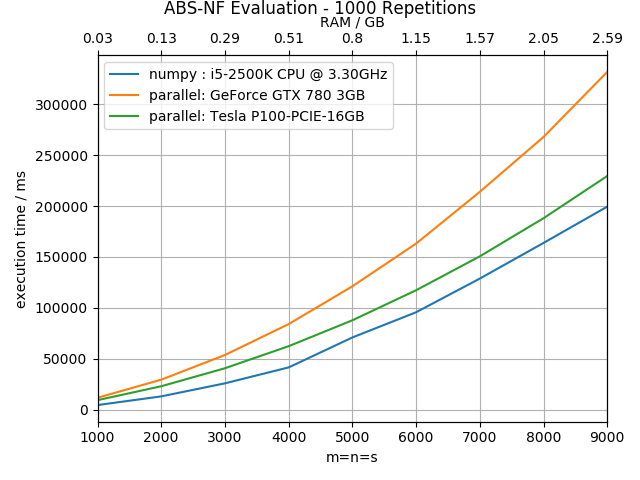
\includegraphics[width=0.6\textwidth]{img/eval_mult_repetition.png}
	\caption{Multiple executions of the evaluate function on different devices}
	\label{eval_1000}
\end{figure}

\subsubsection{Analysis}
The results of the experiment are heavy in favor of the serial implementation.
For small data structures, that completely fit into the global memory of the device, we couldn't get any performance gains through the cuda implementation on given devices. fig \ref{eval_single_repetition} and  fig. \ref{eval_1000}. 
If the data structures get big enoguh such that they don't fit into the global memory of the device, we can expect the performance to be even worse, since the data-transfer time, takes a huge part of the overall runtime. figure \ref{eval_memory}.

We therefore came to the conclusion, that the considerable effort of implementing a parallel version of the eval function is not worth the effort.
\begin{itemize}
	\item Memory Complexity $O(s^2)$
	\item Complexity $O(s^2)$
	\item mempry is bottle neck
	\item no performance gain expected
\end{itemize}

what can be implemented differently? What can be improved?

\subsubsection{Notes}
\begin{itemize}
	\item Double Precision on GTX is nuts
\end{itemize}

